% Source: AESP_466_ClassWork/Supplements/Notes/latex/6.2.5/6.2.5.tex

\documentclass[border=4pt]{standalone}
\usepackage{amsmath,amssymb,amsthm}
\usepackage{graphicx}
\usepackage{tikz}
\usepackage{xcolor}
\usetikzlibrary{arrows.meta,calc,positioning,decorations.markings,patterns,shapes.geometric,angles,quotes}

\definecolor{Garnet}{HTML}{73000A}
\definecolor{USC_Rose}{HTML}{CC2E40}
\definecolor{USC_Blue}{HTML}{466A9F}
\definecolor{USC_Slate}{HTML}{1F414D}
\definecolor{USC_Olive}{HTML}{65780B}
\definecolor{USC_Lime}{HTML}{CED318}
\definecolor{USC_Gold}{HTML}{A49137}
\definecolor{USC_Black90}{HTML}{565556}
\definecolor{USC_Black10}{HTML}{ECECEC}

\newcommand{\vect}[1]{\mathbf{#1}}
\newcommand{\mat}[1]{\mathbf{#1}}
\newcommand{\uvec}[1]{\hat{\mathbf{#1}}}
\newcommand{\transpose}{^{\mkern-1.5mu\mathsf{T}}}
\newcommand{\inv}{^{-1}}
\newcommand{\deriv}[2]{\frac{d #1}{d #2}}
\newcommand{\pderiv}[2]{\frac{\partial #1}{\partial #2}}

\begin{document}
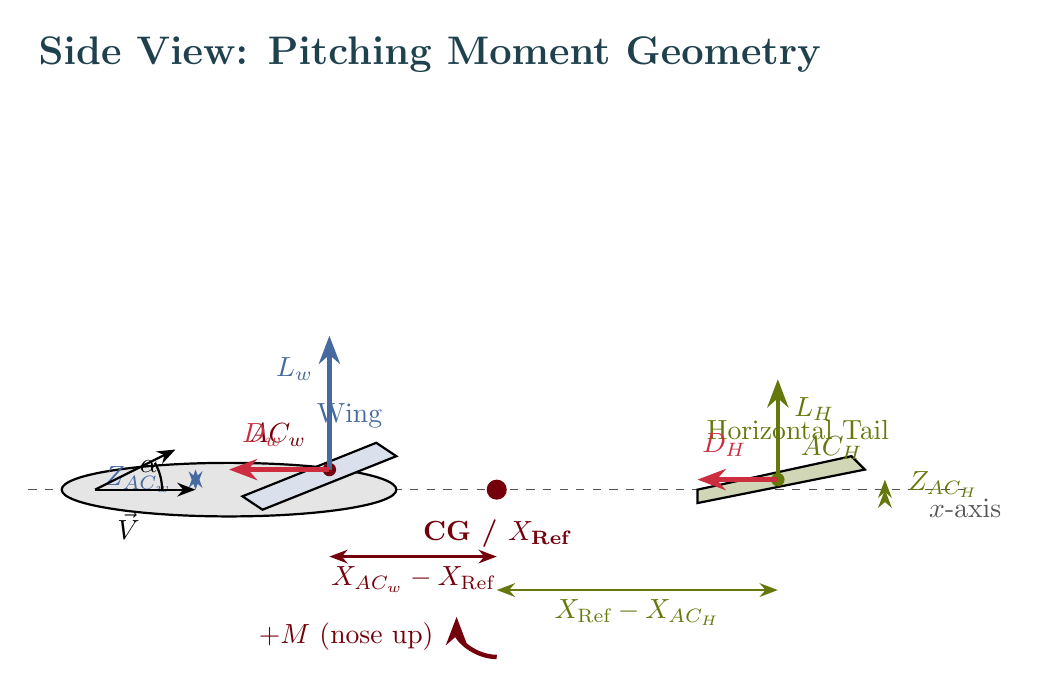
\begin{tikzpicture}[>=Stealth, scale=0.85]
    % Title
    \node[font=\Large\bfseries, USC_Slate] at (4,6.5) {Side View: Pitching Moment Geometry};

    % Horizontal reference line (flight path / x-axis)
    \draw[dashed, USC_Black90] (-2,0) -- (12,0);
    \node[USC_Black90, below] at (12,0) {$x$-axis};

    % Fuselage (simplified)
    \draw[thick, fill=gray!20] (1,0) ellipse (2.5 and 0.4);

    % Wing (at angle showing lift and drag)
    \draw[thick, fill=USC_Blue!20] (1.5,-0.3) -- (3.5,0.5) -- (3.2,0.7) -- (1.2,-0.1) -- cycle;
    \node[USC_Blue] at (2.8,1.1) {Wing};

    % Wing aerodynamic center
    \fill[Garnet] (2.5,0.3) circle (0.1);
    \node[Garnet, above left] at (2.3,0.5) {$AC_w$};

    % Horizontal tail
    \draw[thick, fill=USC_Olive!30] (8,-0.2) -- (10.5,0.3) -- (10.3,0.5) -- (8,0) -- cycle;
    \node[USC_Olive] at (9.5,0.9) {Horizontal Tail};

    % Tail aerodynamic center
    \fill[USC_Olive] (9.2,0.15) circle (0.1);
    \node[USC_Olive, above right] at (9.4,0.3) {$AC_H$};

    % Reference point (CG)
    \fill[Garnet] (5,0) circle (0.15);
    \node[Garnet, below] at (5,-0.3) {\textbf{CG / $X_{\text{Ref}}$}};

    % Wing forces - Lift (perpendicular to flight path)
    \draw[->, ultra thick, USC_Blue] (2.5,0.3) -- (2.5,2.3);
    \node[USC_Blue, left] at (2.4,1.8) {$L_w$};

    % Wing forces - Drag (parallel to flight path)
    \draw[->, ultra thick, USC_Rose] (2.5,0.3) -- (1.0,0.3);
    \node[USC_Rose, above] at (1.5,0.5) {$D_w$};

    % Tail forces - Lift
    \draw[->, ultra thick, USC_Olive] (9.2,0.15) -- (9.2,1.65);
    \node[USC_Olive, right] at (9.3,1.2) {$L_H$};

    % Tail forces - Drag
    \draw[->, ultra thick, USC_Rose] (9.2,0.15) -- (8.0,0.15);
    \node[USC_Rose, above] at (8.4,0.35) {$D_H$};

    % Horizontal moment arm for wing (X_ACw - X_Ref)
    \draw[<->, thick, Garnet] (2.5,-1.0) -- (5,-1.0);
    \node[Garnet, below] at (3.75,-1.0) {$X_{AC_w} - X_{\text{Ref}}$};

    % Horizontal moment arm for tail (X_Ref - X_ACH)
    \draw[<->, thick, USC_Olive] (5,-1.5) -- (9.2,-1.5);
    \node[USC_Olive, below] at (7.1,-1.5) {$X_{\text{Ref}} - X_{AC_H}$};

    % Vertical offset for wing (Z_ACw)
    \draw[<->, thick, USC_Blue] (0.5,0) -- (0.5,0.3);
    \node[USC_Blue, left] at (0.3,0.15) {$Z_{AC_w}$};

    % Vertical offset for tail (Z_ACH)
    \draw[<->, thick, USC_Olive] (10.8,0) -- (10.8,0.15);
    \node[USC_Olive, right] at (11.0,0.08) {$Z_{AC_H}$};

    % Angle of attack indication
    \draw[->, thick] (-1,0) -- (0.5,0);
    \draw[->, thick] (-1,0) -- (0.2,0.6);
    \draw[thick] (0,0) arc (0:30:0.8);
    \node at (-0.2,0.35) {$\alpha$};
    \node[below] at (-0.5,-0.2) {$\vec{V}$};

    % Positive moment direction (nose up)
    \draw[->, ultra thick, Garnet] (5,-2.5) arc (270:180:0.6);
    \node[Garnet, left] at (4.2,-2.2) {$+M$ (nose up)};

\end{tikzpicture}
\end{document}
